\documentclass[../writeup.tex]{subfiles}

\begin{document}  

\section{Clarifications} 
 
\subsection{Structured Light Stereo}

Some relevant reiews are \cite{salviPatternCodificationStrategies2004},\cite{salviStateArtStructured2010} and \href{http://www.sci.utah.edu/~gerig/CS6320-S2013/Materials/CS6320-CV-S2012-StructuredLight-II.pdf}{slides}. A \textit{structured light stereometric system} is similar to a passive stereo system where one of the camera is replaced by a projector. A light source projects light a vertical plane of light that creates a narrow stripe on the scene. The intersection of an illumination plane of known spatial position (corresponds to a projector column) and a line of sight (corresponds to a camera pixel) determines a point. For dense reconstruction of the scene, many images must be taken. To speed up the scanning process, spatially modulated light projector has been suggested, in which multiple illumination planes or rays can be projected simultaneously as part of a single illumination pattern. Spatial-temporal modulation of illumination, i.e. sequentially projecting several patterns, can be used for reliable identification of light planes. To enable acquisition of dynamic scenes, the number of projected patterns used should be as small as possible. Intuitively, the projected pattern impose illusion of texture on the object, increasing the number of correspondences, which enables reconstruction. Structured light stereo is equivalent to (1) solving the correspondence problem and then (2) computing stereo using triangulation.


\paragraph{The Correspondence Problem}

The correspondence problem can be stated simply
\begin{center}
    \textit{
        For each point in the left image, find the corresponding point in the right image
    }
\end{center}
We first note that search space for the corresponding point can be restricted to pixels lying on the epipolar line. Epipolar plane is plane formed from points $p,o_1,o_2$ and epipolar line is intersection of epipolar plane with the image plane.
\begin{figure}[h!]
    \begin{center}
        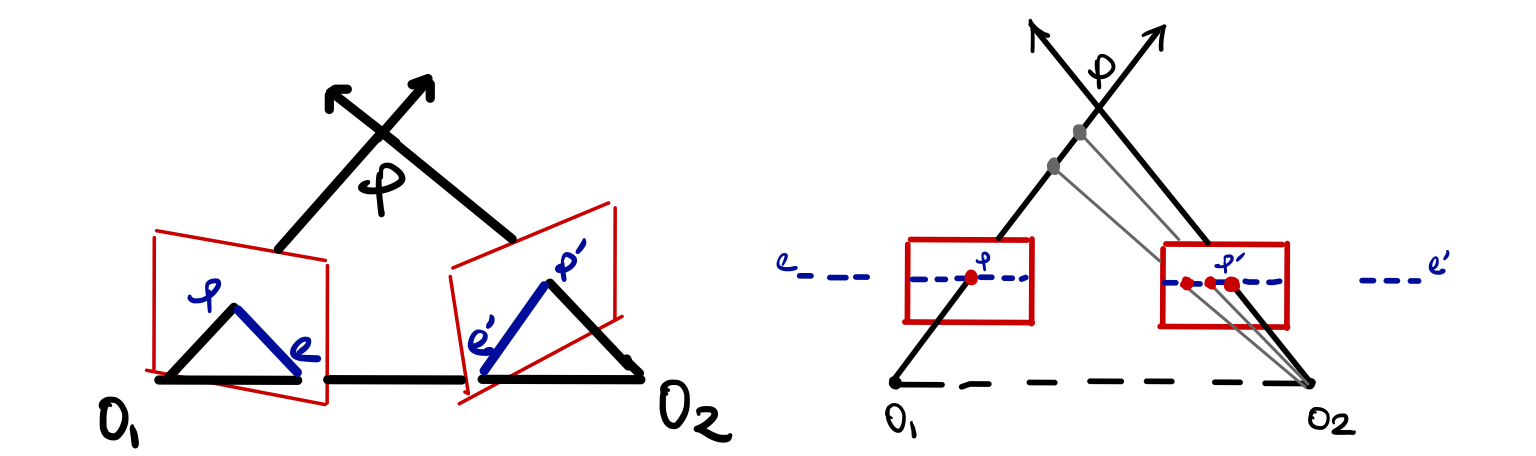
\includegraphics[width=5in]{epipolar_constraint_correspondence}
        \caption{non parallel (left) and parallel (right) camera setup. $pe$ and $p'e'$ are the epipolar lines}
    \end{center}
\end{figure}
For structured light stereo systems, the art of designing robust, fast, reliable coding schemes serves to solve the correspondence problem.


\paragraph{Triangulation}

Given correspondence between projector and camera images, triangulation refers to the process of computing the distance of object relative to camera. Since a 3D point can be obtained by intersecting a ray (pixel of camera image) with a projector plane (a single code), it is necessary to encode a single axis in projected image to ensure unique reconstruction. 
\begin{figure}[h!]
    \begin{center}
        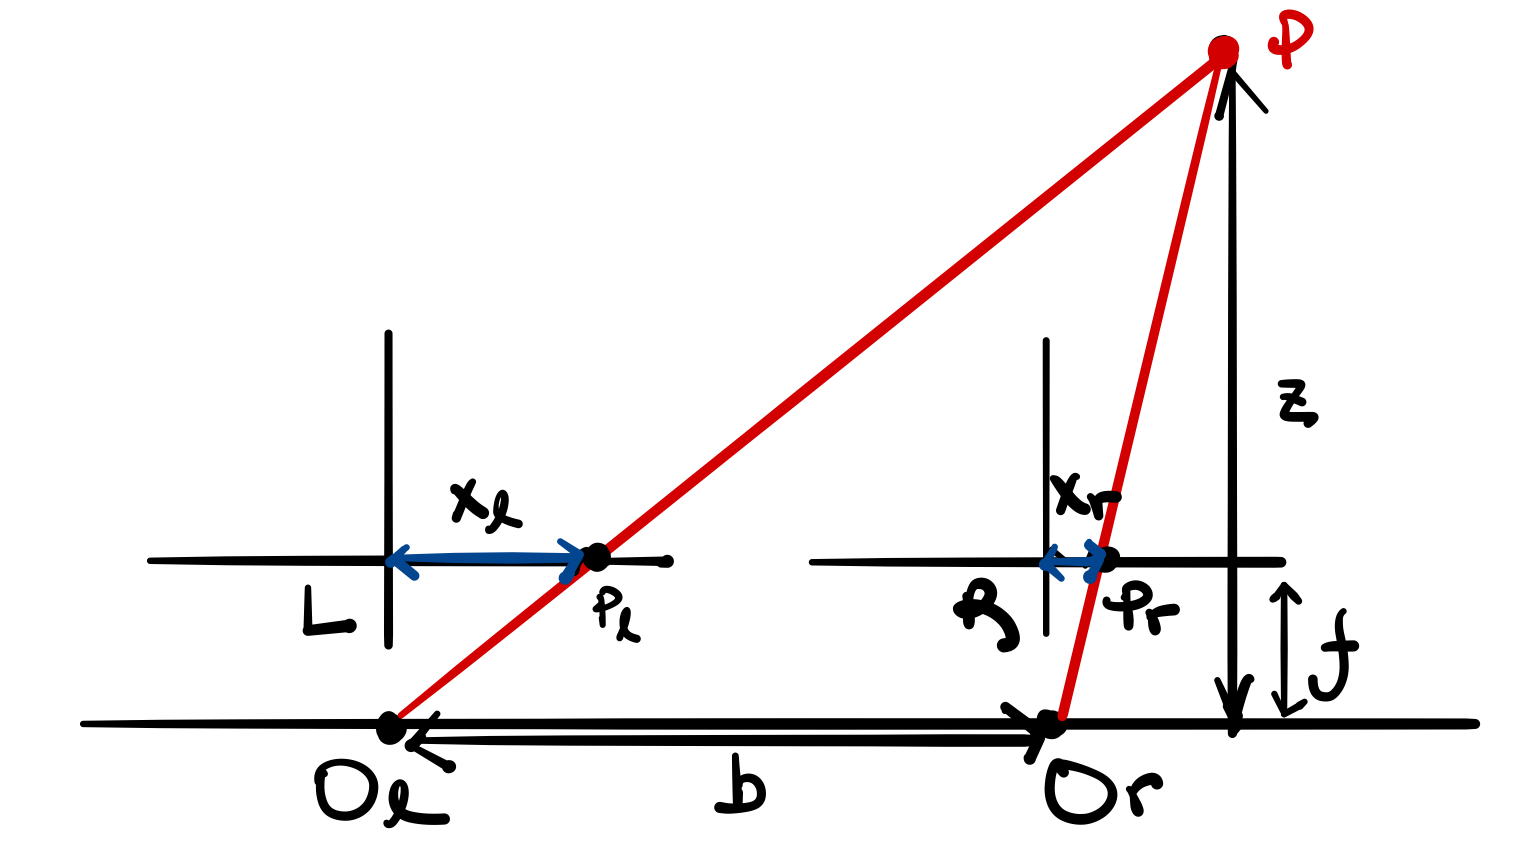
\includegraphics[width=3in]{parallel_camera}
        \caption{parallel-calibrated binocular stereo}
    \end{center}
\end{figure}
\noindent \textit{disparity} is the displacement between points of a conjugate pair $p_l,p_r$ (points in different images of projection of same point in the scene) when the two images are superimposed. In the context of parallel calibrated cameras, disparity is inversely proportional to depth, when baseline $b$ and focal length $f$ are known
\begin{align*}
    \frac{b}{z} = \frac{b + x_l - x_r}{z-f}
    \quad\text{implies}\quad
    z = \frac{bf}{x_l-x_r}
\end{align*}

\subsection{Structured Light Coding}

The goal of structured light coding is to find coding schemes (maps pattern intensity to indices of the projector light planes) that enables robust, reliable algorithms for finding correspondence.


\paragraph{Horn \& Kiryati} 

This paper generalizes Gray code to n-ary code in order to reduce the number of patterns that needs to be projected, ($L^K$ instead of $2^K$ code words) \cite{hornOptimalStructuredLight1997}. The authors draw inspirations from communication theory, where the projector projects unique temporal codes, received at each image plane through a noisy channel and subsequently decoded. Let there be $K$ patterns and $L$ code words (distinct planes of light), we want to encode the indices of vertical light planes $x\in [L]$ using some encoding scheme $f:[L] \to \R^K$ such that the nearest neighbor decoding $\hat{x}(y) = \argmin_{x\in [L]} ( f(x)-y )$ of a normalized noisy observation $y\in\R^K$ minimizes the probability of depth estimation error. Given the forwarding model,
\begin{align*}
    \ry = f(\rx) + \rn
    \quad\quad\text{where}\quad\quad
    \rx 
        &\sim \text{Cat}(1/L)
    \quad
    \rn
        \sim p_{\rn}
\end{align*}
implying $\ry|\rx=x\sim p_{\rn}(y - f(x))$. We want to minimize the probability of depth estimation error, which roughly proportional to difference between true index $x$ of the plane of light and the estimated index $\hat{x}$,
\begin{align*}
    \text{minimize}_{f}\;\; \pb{
        \E_{\rx,\ry} \left[ (x-\hat{x}(y))^2 \right]
        = \sum_{x=1}^L p_{\rx}(x) \int p_{\ry|\rx}(y|x) (x - \hat{x}(y))^2 dy
        \propto \sum_{x=1}^L \int (x-\hat{x}(y))^2 p_{\rn}(y-f(x)) dy
    }
\end{align*}
This optimization problem is hard. The paper suggest the use of space filling curves as the encoding function and established that Gray code is a special limiting case of the space filling curve. Note here we assume there is no \textit{mutual illumination}, i.e. there is no interval reflection and so the projected codes $f(x)$ is proportional to observation $y$. 

\paragraph{Phase Shifting}

Phase shifting is a particular coding method whereby the projector column coordinates are encoded as the (absolute) phase of a spatial sinusoidal pattern. Note we want to encode column coordinates because we only need to search along the horizontal epipolar lines. Let $N$ be number of columns to be encoded. When the scene is projected with a cosine pattern of period $T$ (measured in number of pixels) and therefore frequency $f=\frac{1}{T}$, an idealized image formation model for any pixel is 
\begin{align}
    I 
        = I_0 + A\cos\left( \Phi \right)
        = I_0 + A\cos\left( \phi \right)
    \label{eq:phase_shift_image_formation_one_pixel}
\end{align}
where $I_0$ is the pixel intensity when no projection is used; $I$ is the pixel intensity measured; $A$ is amplitude (albedo/reflectance) of the signal; $\Phi = 2\pi f x = 2\pi n + \phi \in [0, 2\pi f N]$ for some number of period $n\in\N$ is the absolute phase, $\phi \in [0,2\pi]$ is the relative phase. When measured w.r.t. number of pixels, $x$ is the corresponding absolute phase and $\tilde{x}$ the corresponding relative phase, satisfying
\begin{align}
    x = Tn + \tilde{x}
    \qquad\text{or}\qquad
    x \equiv \tilde{x} \mod{T}
\end{align}
where $\tilde{x} = \frac{T \phi}{2\pi}$. In (\ref{eq:phase_shift_image_formation_one_pixel}), $I_0,A,\phi$ are unknown and so $\phi$ cannot be determined. To solve for $\phi$, phase shifting method projects $K$ sinusoidal patterns of same frequency, each shifted by $\varphi_k = \frac{2\pi (k-1)}{K}$ for $k=1,\cdots,K$. Thereby obtaining a system of $K$ equations in 3 unknowns. 
\begin{align}
    I_k = I_0 + A\cos\left(\phi + \varphi_k \right)
    \qquad\text{for}\qquad
    k = 1,\cdots,K
    \label{eq:phase_shift_image_formation_one_pixel_shifted}
\end{align}
Although $K=3$ suffices, larger values of $K$ makes determination of relative phase $\phi$ more robust to noise. We determine $\phi$ using least squares
\begin{align}
    \text{minimize}_{\phi}\;\;\pb{
        \epsilon(\phi,I_0,A) := 
            \sum_{k=1}^{K} \pb{
                I_k - \left(
                    I_0 + A\cos\left( \phi + \varphi_k \right)
                \right)
            }^2
    }
    \label{eq:phase_shifting_least_squares}
\end{align}
Similar to appendix in \cite{morenoEmbeddedPhaseShifting2015} and results shown in \cite{pribanicEfficientMultiplePhase2010,morenoEmbeddedPhaseShifting2015}, we can show the following
\begin{align*}
    0
        = \frac{\partial \epsilon}{\partial \phi}
        &= 2A \sum_{k=1}^K I_i\sin \left( \phi + \varphi_k \right)
        \propto \cos(\phi) \sum_{k=1}^K I_k \sin(\varphi_k) + \sin(\phi) \sum_{k=1}^{K} I_k \cos(\varphi_k) \\
    \phi
        &= \tan^{-1}\pb{
            -
            \frac{
                \sum_{k=1}^K I_k \sin(\varphi_k)
            }{
                \sum_{k=1}^K I_k \cos(\varphi_k)
            }
        }
\end{align*}
An alternative formulation as mentioned in \cite{guptaMicroPhaseShifting2012}, we can write (\ref{eq:phase_shift_image_formation_one_pixel_shifted}) as a linear system of equations
\begin{align*}
    I_k
        &= I_0 + A\cos(\phi)\cos(\varphi_k) - A\sin(\phi)\sin(\varphi_k)
        = \begin{bmatrix}
            1 & \cos(\varphi_k) & -\sin(\varphi_k)
        \end{bmatrix}
        \begin{bmatrix}
            I_0 \\ A\cos(\phi) \\ A\sin(\phi)
        \end{bmatrix} \\
    \underbrace{
        \begin{bmatrix}
            I_1 \\ \vdots \\ I_K
        \end{bmatrix}
    }_{\bI}
        &= 
        \underbrace{
            \begin{bmatrix}
                1 & \cos(\varphi_1) & -\sin(\varphi_1) \\
                \vdots & \vdots & \vdots \\
                1 & \cos(\varphi_K) & -\sin(\varphi_K) \\
            \end{bmatrix}
        }_{\bM}
        \underbrace{
            \begin{bmatrix}
                I_0 \\ A\cos(\phi) \\ A\sin(\phi)
            \end{bmatrix}
        }_{\bu}
\end{align*}
and solve for $\bu$ using least squares,
\begin{align}
    \text{minimize}_{\bu}\;\;
        \norm{\bI-\bM\bu}_2^2
    \label{eq:phase_shifting_least_squares_u}
\end{align}
The relative phase is then given by
\begin{align*}
    \phi 
        = \cos^{-1}\left( \frac{\bu_2}{A} \right)
    \qquad\text{where}\qquad
    A
        = \sqrt{\bu_2^2 + \bu_3^2}
    \quad\text{and}\quad
    \bu
        = M^{\dagger} \bI
\end{align*}
Note the optimization problem formulated in (\ref{eq:phase_shifting_least_squares},\ref{eq:phase_shifting_least_squares_u}) are not equivalent. \textit{phase unwrapping} aims to recover absolute phase $x$ from relative phase $\tilde{x}$, which is non-trivial unless $T\geq N$. One particular choice of phase unwrapping method relies results in number theory \cite{gushovAutomaticProcessingFringe1991}. The idea is to project patterns whose periods $T_1,\cdots,T_F$ are relative co-prime, each shifted by $K$ times such that relative phase $\tilde{x}_1,\cdots,\tilde{x}_F$ can be solved using (\ref{eq:phase_shifting_least_squares}) or (\ref{eq:phase_shifting_least_squares_u}), from which we can use the Chinese Reminder Theorem to solve the following system of congruences
\begin{align}
    x
        &= \tilde{x}_1 \mod{T_1} 
        \nonumber \\
    &\vdots
        \nonumber \\
    x
        &= \tilde{x}_F \mod{T_F} 
    \label{eq:phase_shifting_congruence_system}
\end{align}
Intuitively, projecting $F$ spatial sinusoids with period $T_1,\cdots,T_F$ with different frequency emulates the projection of a low frequency spatial sinusoid with period $T = T_1\times \cdots\times T_F$, shown in Figure (\ref{fig:phase_shifting_emulate_low_freq}).
\begin{figure}[h!]
    \begin{center}
        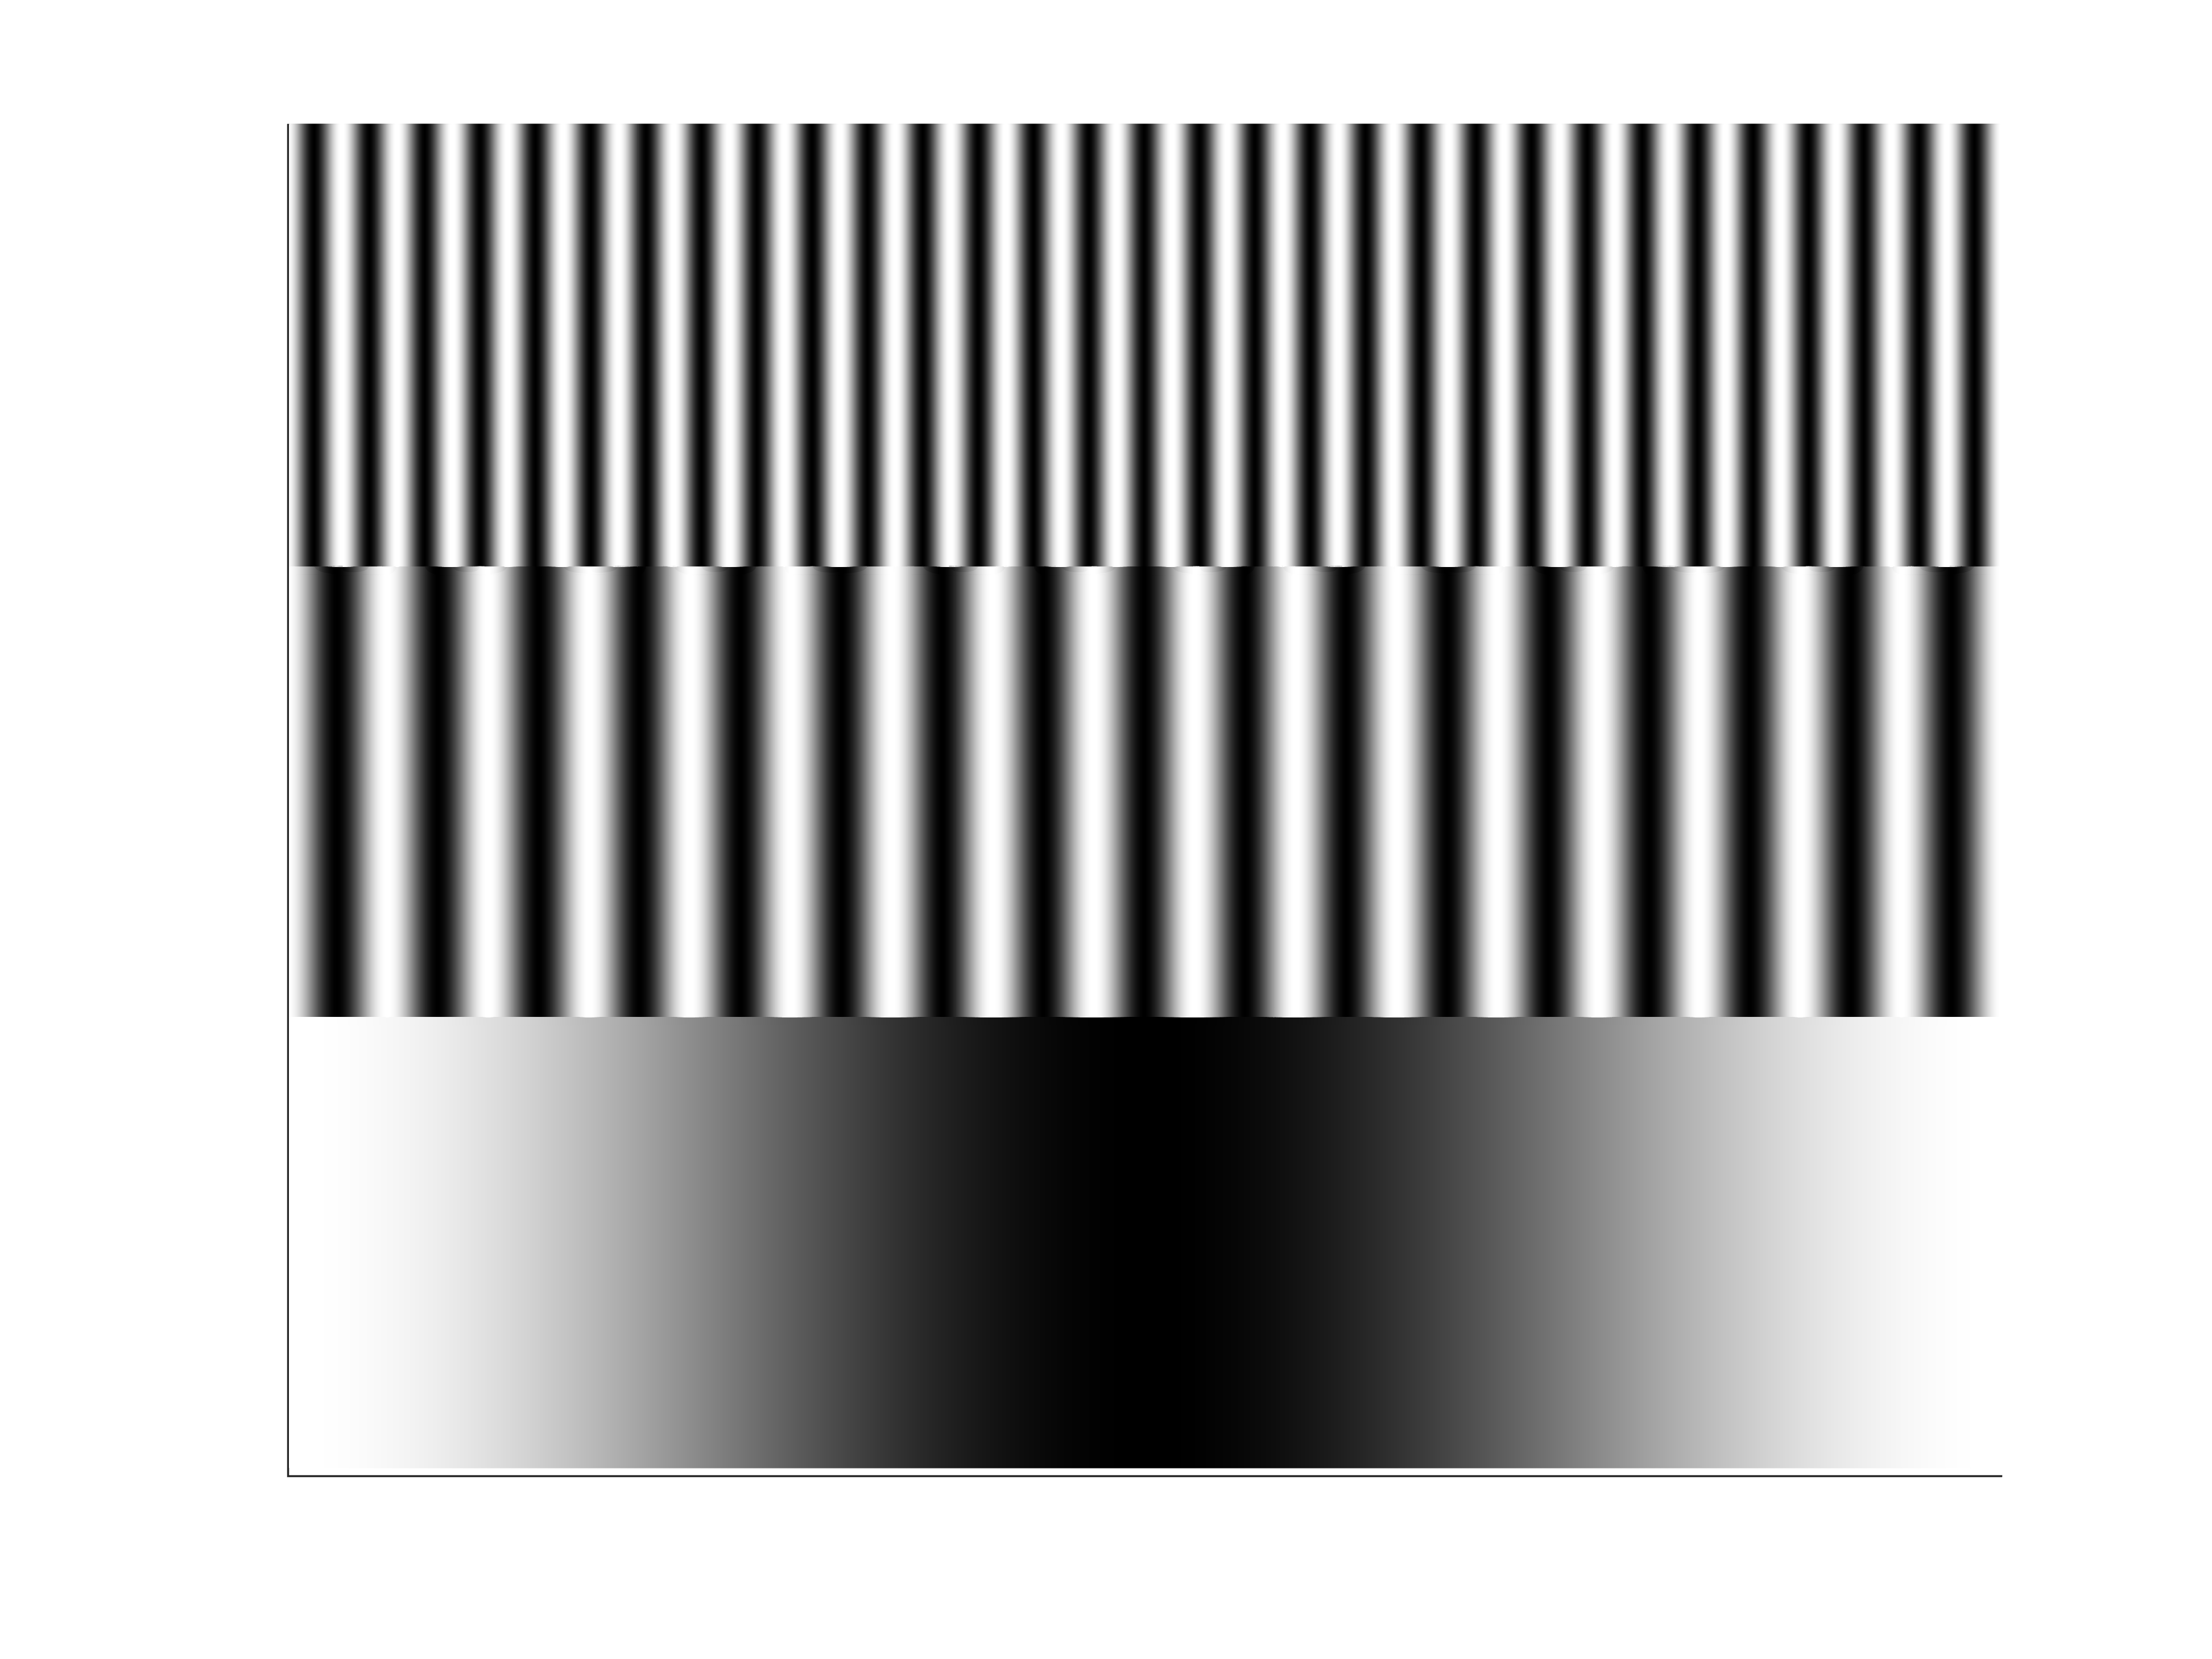
\includegraphics[height=1in,width=6in]{phase_shifting_chinese_reminder_lower_freq}
    \end{center}
    \caption{Two sinusoids with $T_1=17,T_2=31$ emulates a low frequency sinusoid with $T=527$}
    \label{fig:phase_shifting_emulate_low_freq}
\end{figure}
As specified in \cite{guptaMicroPhaseShifting2012} and experimented in Figure (\ref{fig:phase_shifting_not_robust_to_noise}), phase unwrapping is unstable when the relatives phases $\tilde{x}_1,\cdots,\tilde{x}_F$ are noisy.
\begin{figure}[h!]
    \begin{center}
        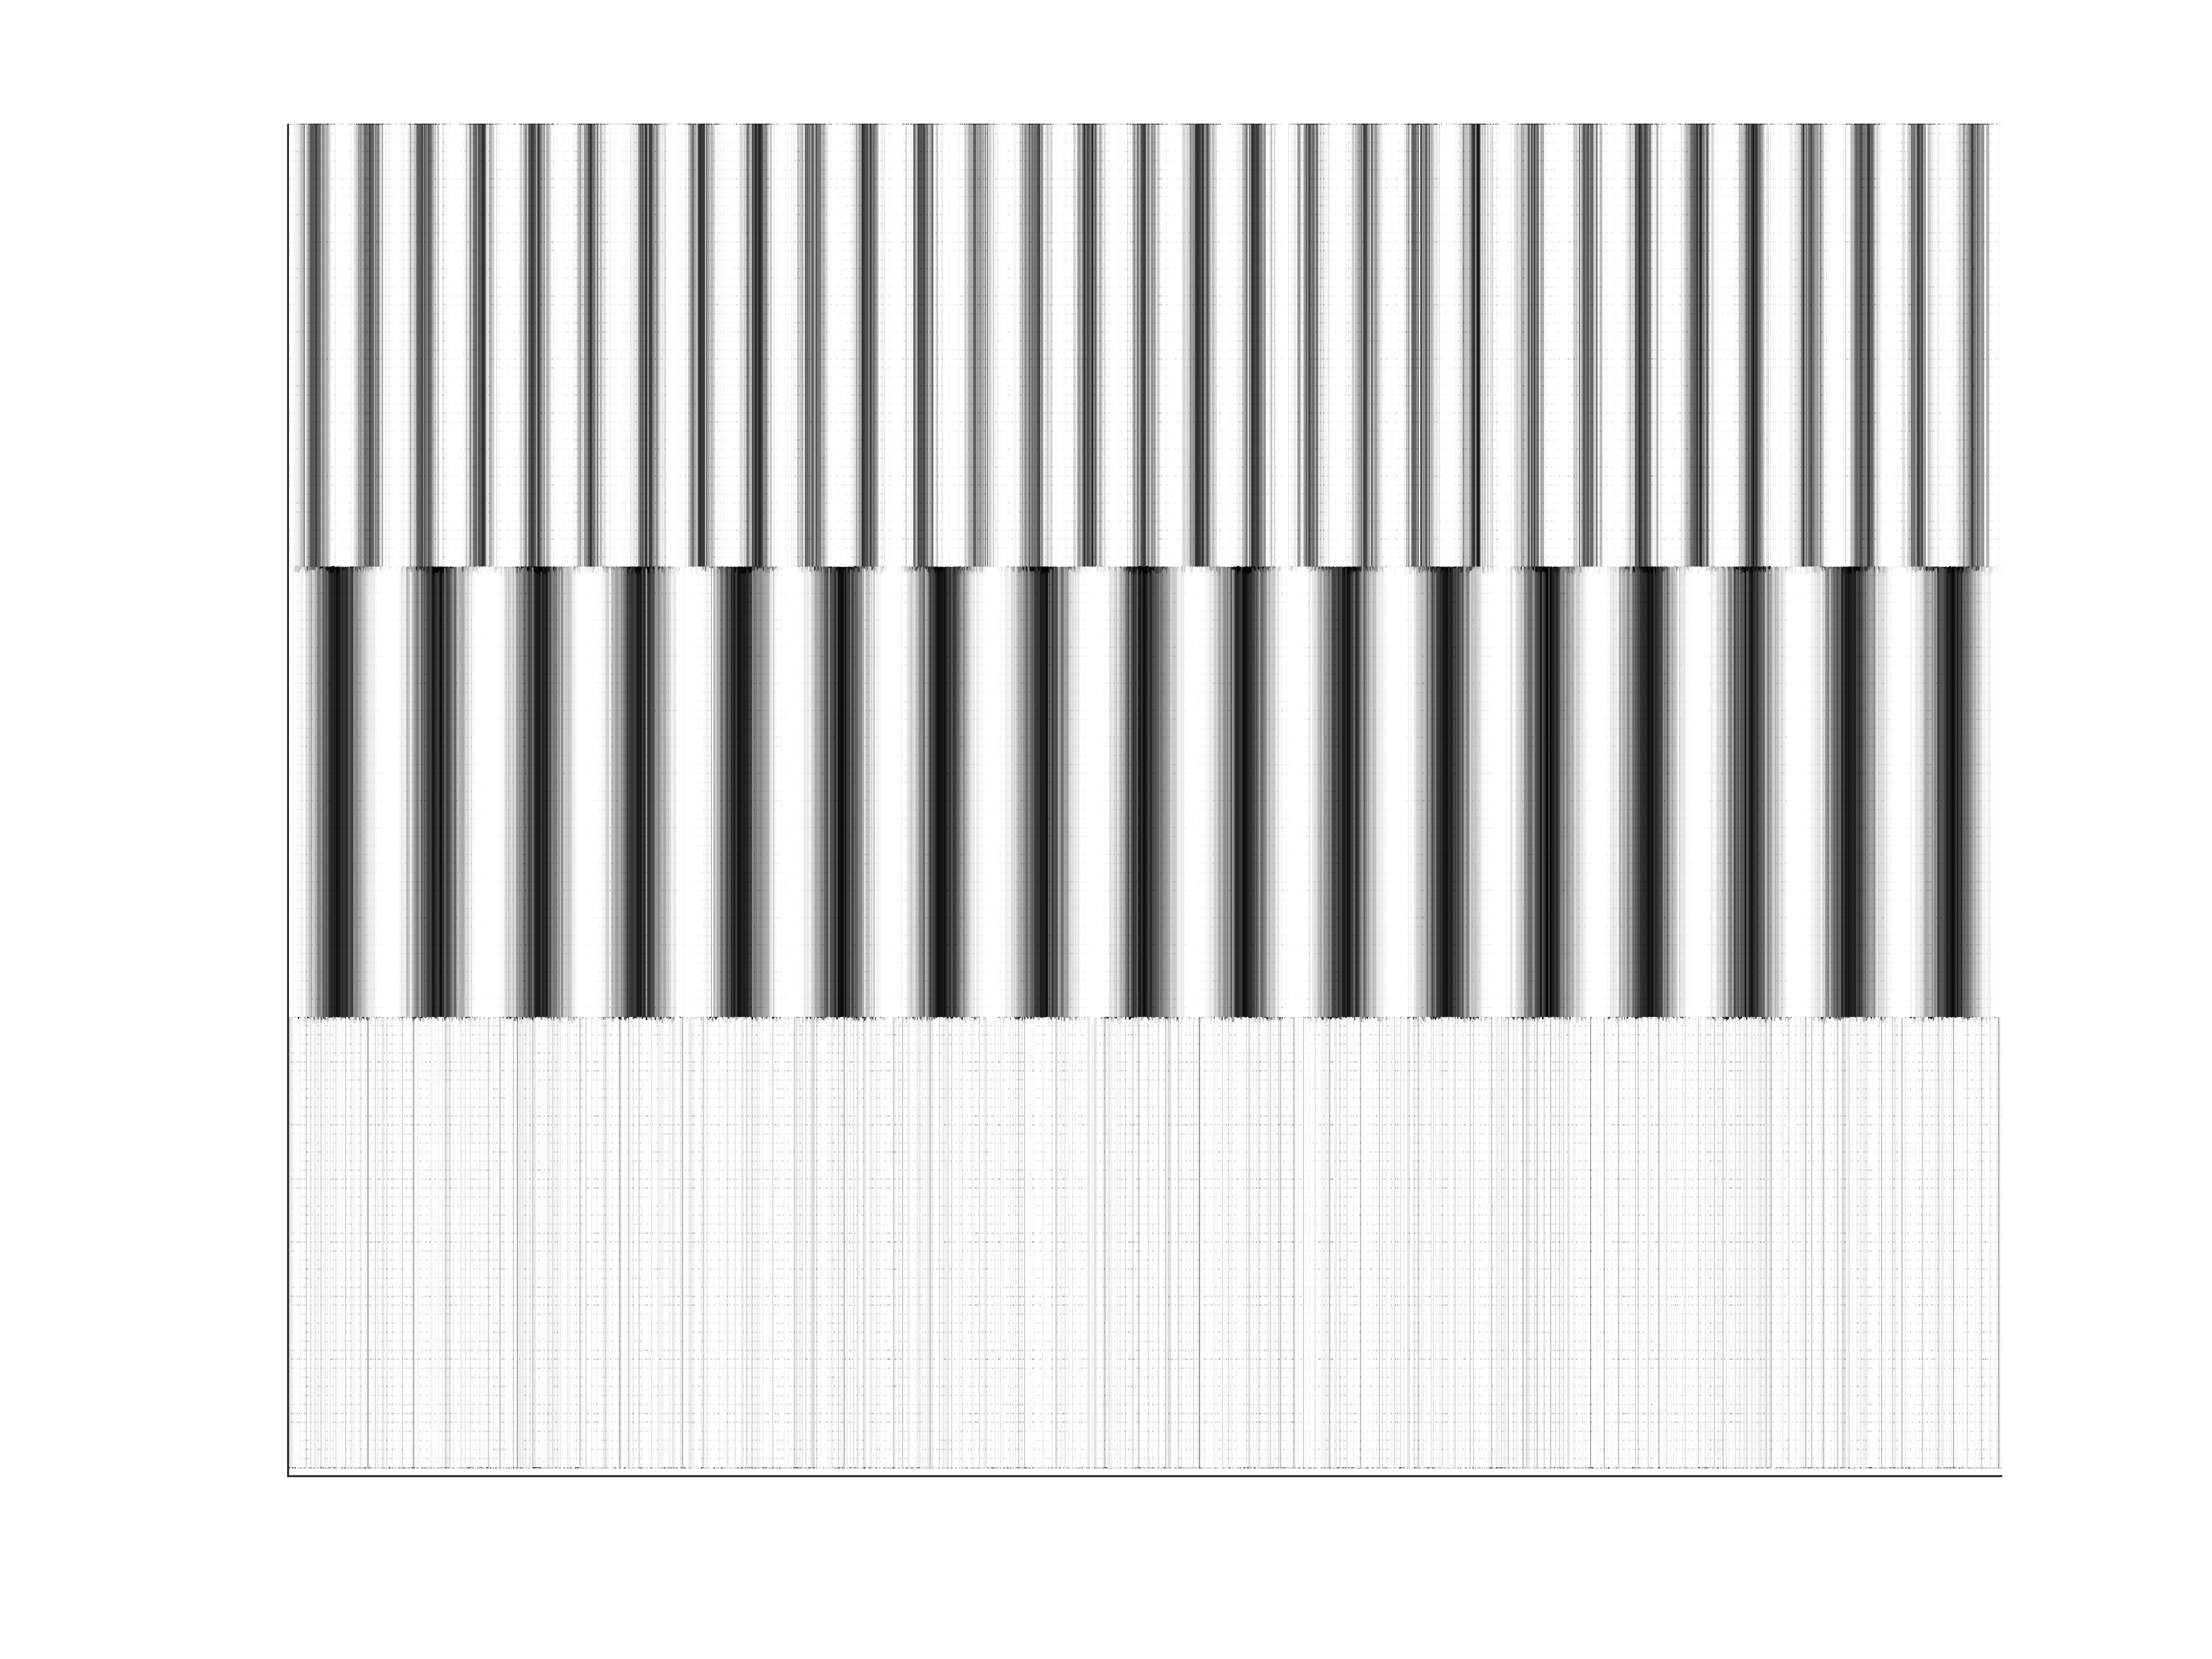
\includegraphics[height=1in,width=6in]{phase_shifting_chinese_reminder_lower_freq_noisy}
    \end{center}
    \caption{When relative phase $\tilde{x}_1,\tilde{x}_2$ are corrupted with i.i.d. additive Gaussian noise $\sN(\boldsymbol{0},0.1 \cdot \textsf{range}(\tilde{x}) \cdot \bI)$, phase unwrapping is unable to recover the absolute phase $x$ robustly.}
    \label{fig:phase_shifting_not_robust_to_noise}
\end{figure}
Simple application of medium filtering of the relative phase does not seem to help with phase unwrapping. Wavelet denoising with \texttt{wdenoise} seems to help to a limited extend, as shown in Figure (\ref{fig:phase_shifting_chinese_reminder_lower_freq_noisy_wdenoiser})
\begin{figure}[h!]
    \begin{center}
        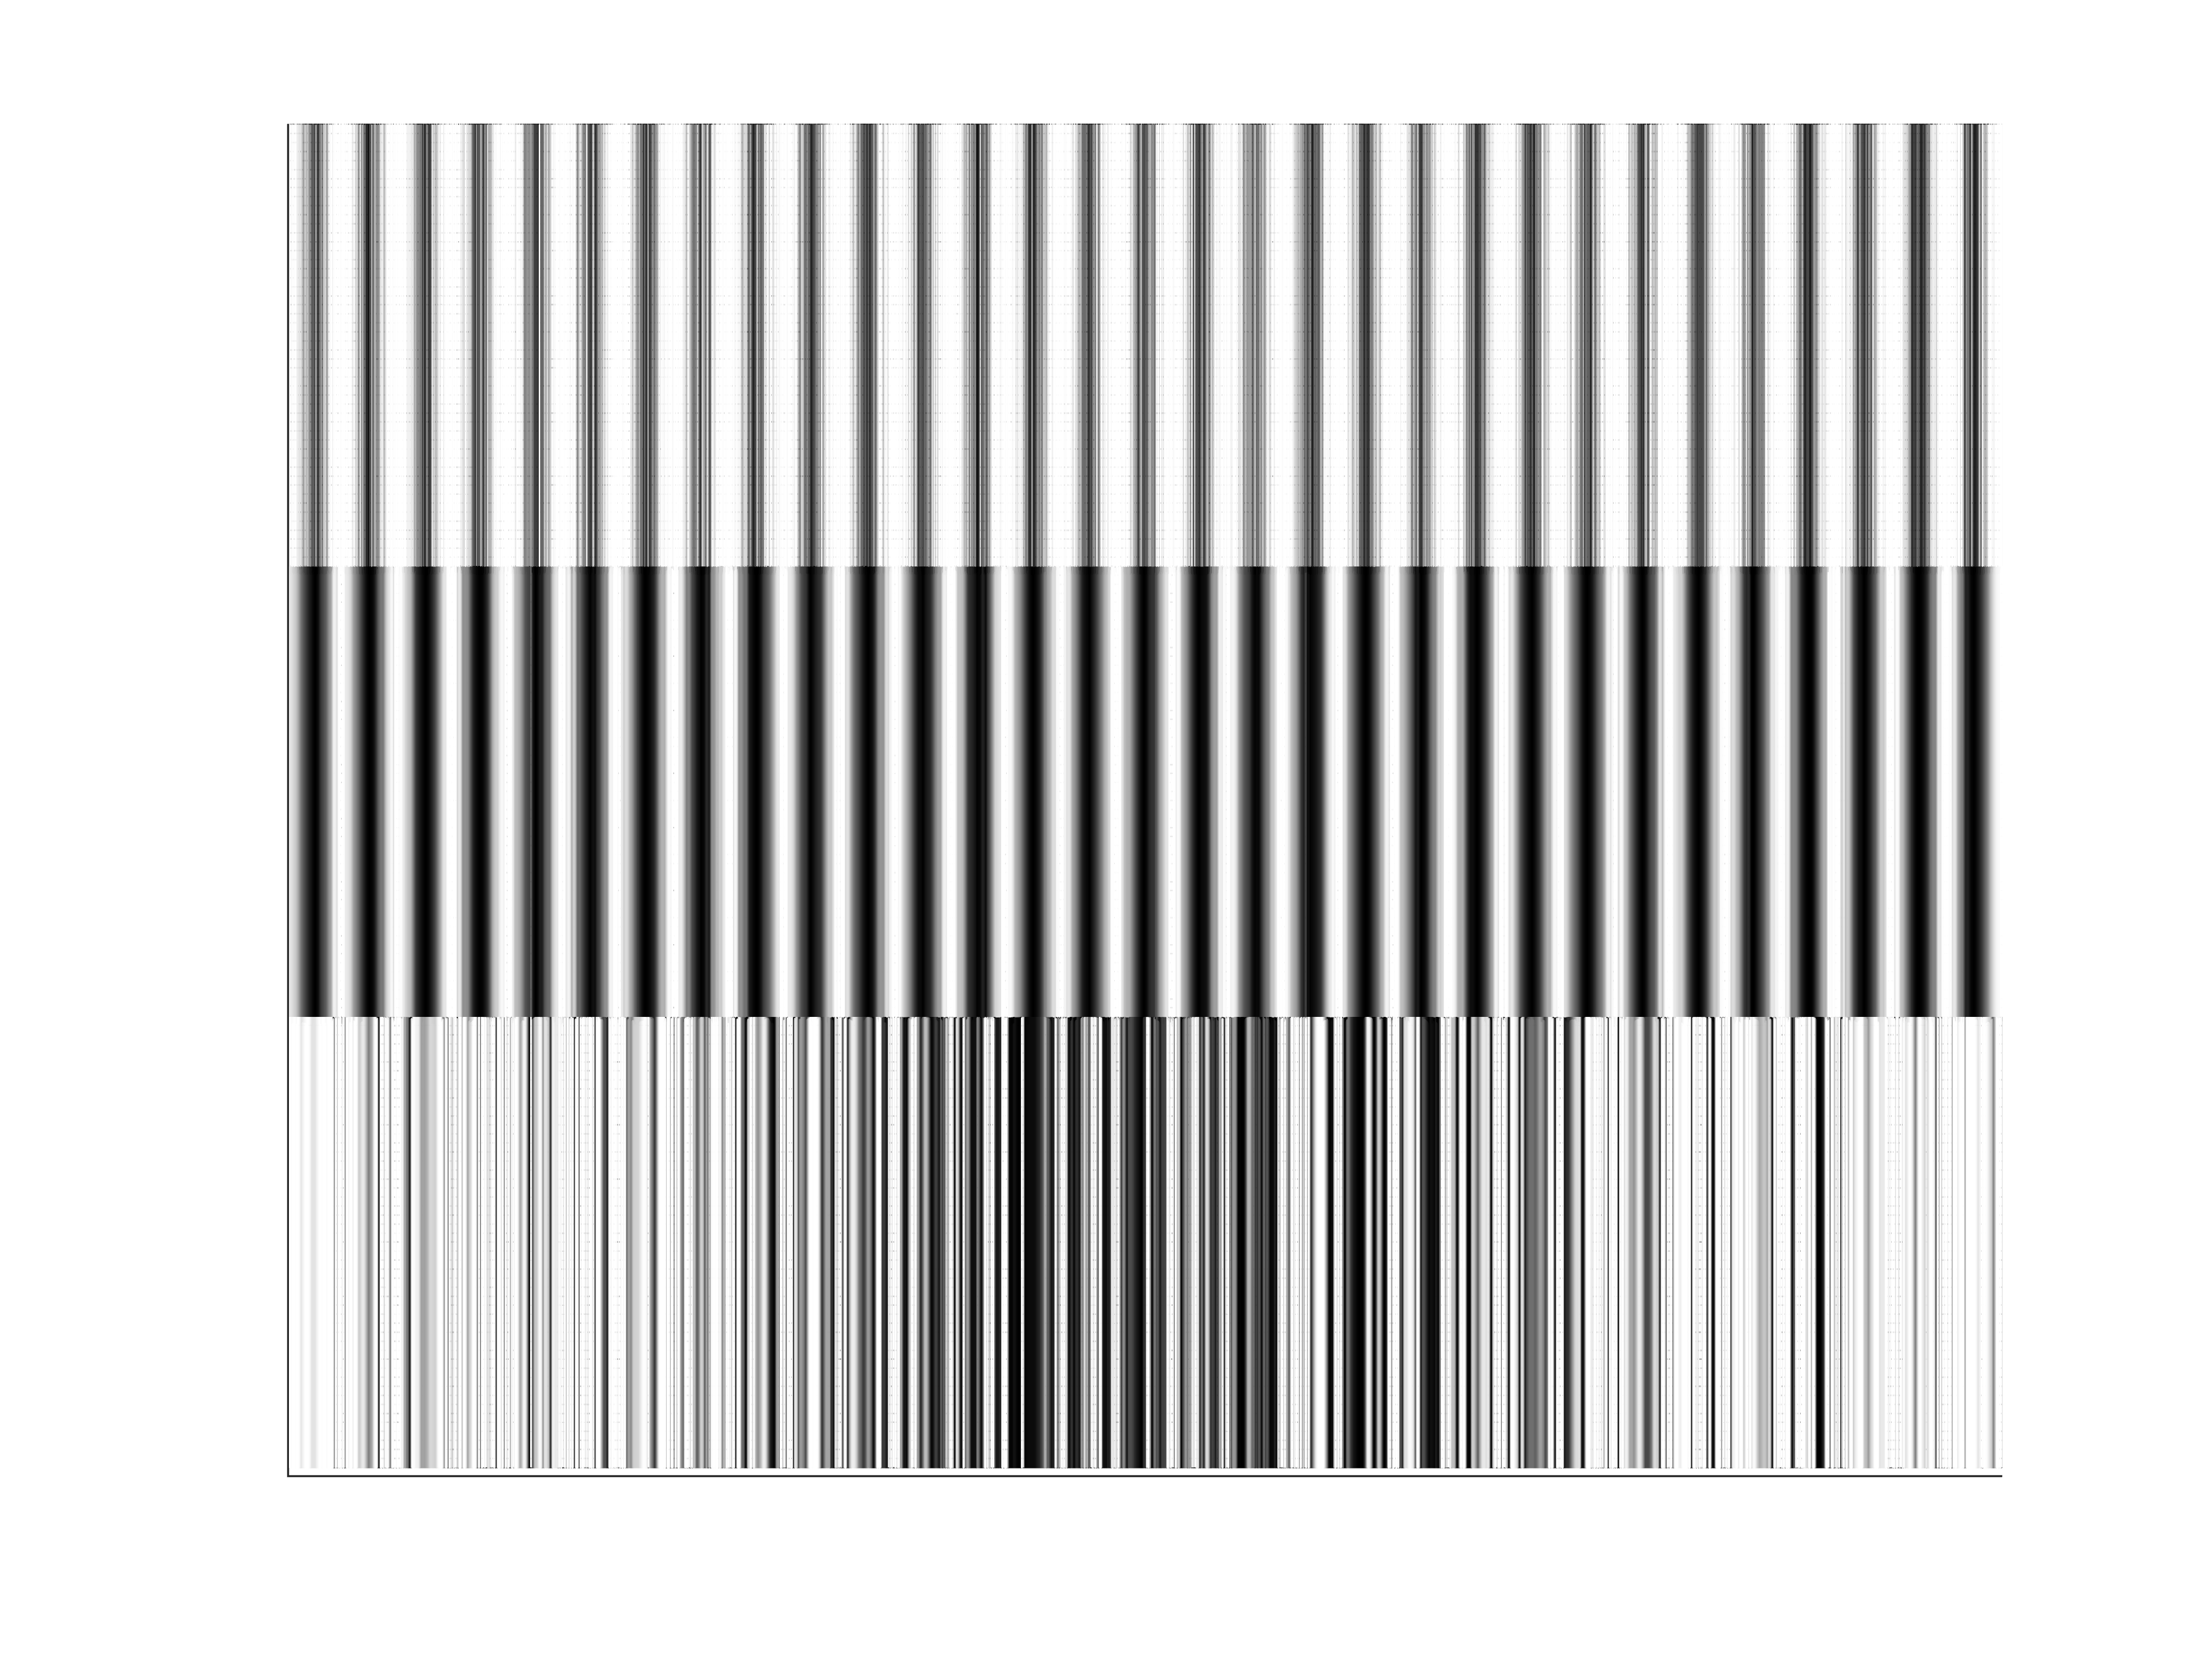
\includegraphics[height=1in,width=6in]{phase_shifting_chinese_reminder_lower_freq_noisy_wdenoiser}
    \end{center}
    \caption{$\tilde{x}_1$ and wavelet denoised $\tilde{x}_1$ ($x_2,\tilde{x}_2$ not shown) helps with phase unwrapping to some extend}
    \label{fig:phase_shifting_chinese_reminder_lower_freq_noisy_wdenoiser}
\end{figure}



\newpage

\subsection{Image Priors} 

The choice of regularization has been an important research topic in image processing. Handcrafted priors have been successful in a number of different image recovery tasks. For example, we can choose to enforce task-specific priors: (1) the sparsity of $\bx$ with $\ell$-1 norm in image deblurring \cite{beckFastIterativeShrinkageThresholding2009} (2) total variation in image denoising \cite{buadesNonlocalImageMovie2008} (3) cross-channel correlation in color image demosaicing \cite{malvarHighqualityLinearInterpolation2004} (4) dark channel prior in image dehazing \cite{fattalSingleImageDehazing2008}, etc. More exhotically, randomly initialized neural network can inject inductive bias to the optimization and act as image priors. \cite{ulyanovDeepImagePrior2017}

$ $\\
In addition to hand-crafted priors, there has been interest in algorithm induced priors. Alternating direction method of multipliers (ADMM) is a common convex optimization method for inverse problem where the objective function is separable with respect to the \textit{data term} and the \textit{regularizer}. Each primal update involves an evaluation of a proximal operator, which can be interpreted as performing denoising on some iterate. \cite{venkatakrishnanPlugandPlayPriorsModel2013,heideFlexISPFlexibleCamera2014,chanAlgorithmInducedPriorImage2016} proposed plug-and-play priors where the choice of regularization is implicitly specified by the denoiser used. \cite{romanoLittleEngineThat2016} proposed an explicit laplacian-based expression for the regularizer and generalizes the method to a number of different iterative optimization algorithms.

$ $\\
The convergence of plug-and-play ADMM is studied by a number of papers. \cite{chanPlugandPlayADMMImage2016} showed fixed point convergence of plug-and-play ADMM. \cite{romanoLittleEngineThat2016} showed convergence of the algorithm under some mild conditions of the denoiser, which are satisfied by some state of the art denoisers like \textit{Block-matching and 3D filtering
 (BM3D)} \cite{dabovImageDenoisingSparse2007} and \textit{Trainable Nonlienar Reaction Diffusion (TNRD)} \cite{chenTrainableNonlinearReaction2017}. Most recently, \cite{ryuPlugandPlayMethodsProvably2019} established convergence given that the denoising network satisfy certain Lipschitz condition.

$ $\\ 
Some proposed to learn proximal operator from data. \cite{meinhardtLearningProximalOperators2017} used a CNN denoiser \cite{zhangGaussianDenoiserResidual2017}. Instead of substituting the proximal operator with a denoiser, \cite{changOneNetworkSolve2017} learns a projection mapping to the space of natural images by training a single neural network and showed impressive results on a number of different linear inverse problems.



\end{document}
